\begin{frame}{Bagging}
    \begin{itemize}
        \item Recall that given a set of $n$ independent observations $Z_1 , \cdots , Z_n$ , each with $Var(Z_i) = \sigma^2$, then $Var(\bar{Z}) = \sigma^2/n$. \pause \\ 
        $\rightarrow$ \textcolor{blue}{Averaging a set of observations reduces variance}.\pause 

        \item We use this idea to do resampling with replacement (bootstrap sample) for the training dataset. \pause 

  \end{itemize}
\end{frame}



\begin{frame}{Bagging}

\footnotesize

\begin{columns}[T]

\column{0.5\linewidth}

        \textbf{For regression:} \\ \pause 
        \begin{itemize}
            \item We generate $B$ different bootstrapped training sets. \pause
            \item Train the model on the $b$th bootstrapped training set % in order to get $\hat{f}^{*b}(x)$. \pause 
            \item  Average all the predictions. \pause 
%        \begin{equation*}
%            \hat{f}_{bag}(x) = \frac{1}{B} \sum_{b=1}^B \hat{f}^{*b}(x).
%        \end{equation*} \pause 

        \end{itemize}
    
        \begin{figure}
            \centering
            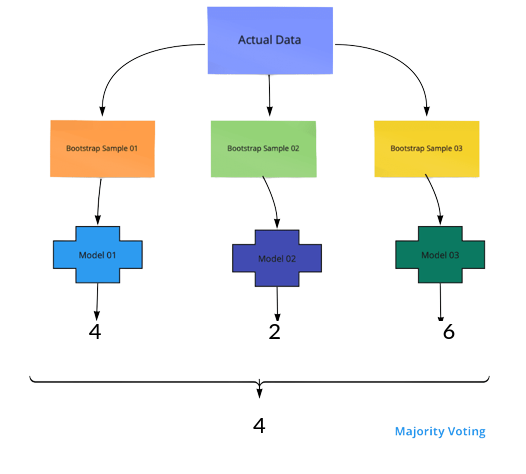
\includegraphics[height=4cm]{bagging-boosting/bagging-regress.png}
        \end{figure} \pause 

\column{0.5\linewidth}


    \textbf{For classification}:\\ \pause 

    \begin{itemize}
        \item We generate $B$ different bootstrapped training sets. \pause
        \item Record the class predicted by each of the $B$ trees.  \pause
        \item Take the \textit{majority vote} as the prediction. \pause
    \end{itemize}

     \begin{figure}
            \centering
            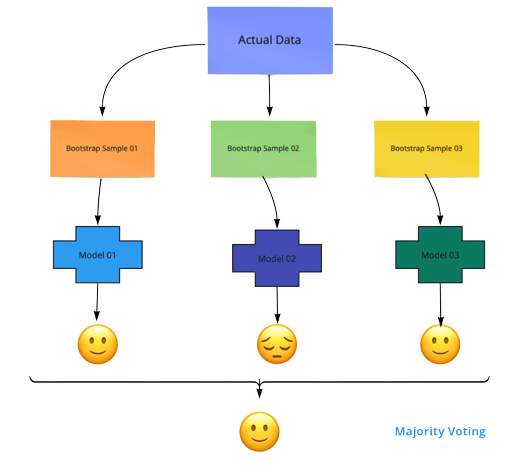
\includegraphics[height=4cm]{bagging-boosting/bagging-class.png}
    \end{figure} 
    

    
\end{columns}


\end{frame}


\begin{frame}{Bagging}{Out-of-Bag Error Estimation}

    \begin{itemize}
        \item On average, each bagged tree makes use of around $2/3$ of the observations. \pause 
        \item The remaining $1/3$ of the observations not used to fit a given bagged tree are referred to as the \textbf{out-of-bag (OOB) observations}. \pause 
        \item We can predict the response for the $i$th observation using each of the trees in which that observation was OOB.  \pause 
        \item The final prediction is then the average predicted responses (for regression) or the majority vote (for classification). \pause 
        \item This leads to a single OOB prediction for the $i$th observation. \pause 
        \item The resulting OOB error is a valid estimate of the test error for the bagged model. 
        
    \end{itemize}

    
\end{frame}

\begin{frame}{Bagging}{Out-of-Bag Error Estimation}

\begin{figure}
    \centering
    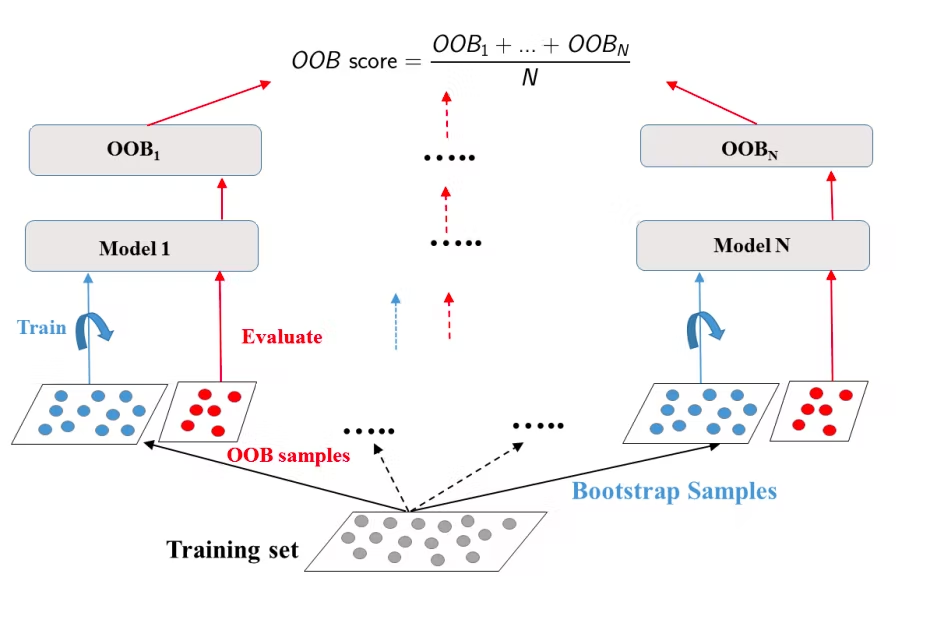
\includegraphics[height=7cm]{bagging-boosting/oob.png}
\end{figure}
    
\end{frame}

\begin{frame}{Bagging}{Variable importance measures}

One can obtain an overall summary of the importance of each predictor.  \pause 

\begin{columns}[T]

\column{0.5\linewidth}

        \textbf{For regression:} \\ \pause 
        \begin{itemize}

        \item We record the total amount that the $RSS$ is decreased due to splits over a given predictor, averaged over all $B$ trees. \pause 
        
        \item A large value indicates an important predictor. \pause 

        \end{itemize}
    
 

\column{0.5\linewidth}


    \textbf{For classification}:\\ \pause 

    \begin{itemize}

    \item We add up the total amount that the Gini index is decreased by splits over a given predictor, averaged over all $B$ trees. \pause 

    \item A small value indicates an important predictor.

    \end{itemize}

 
    
\end{columns}

    
\end{frame}